\begin{figure}[!htbp]
\centering
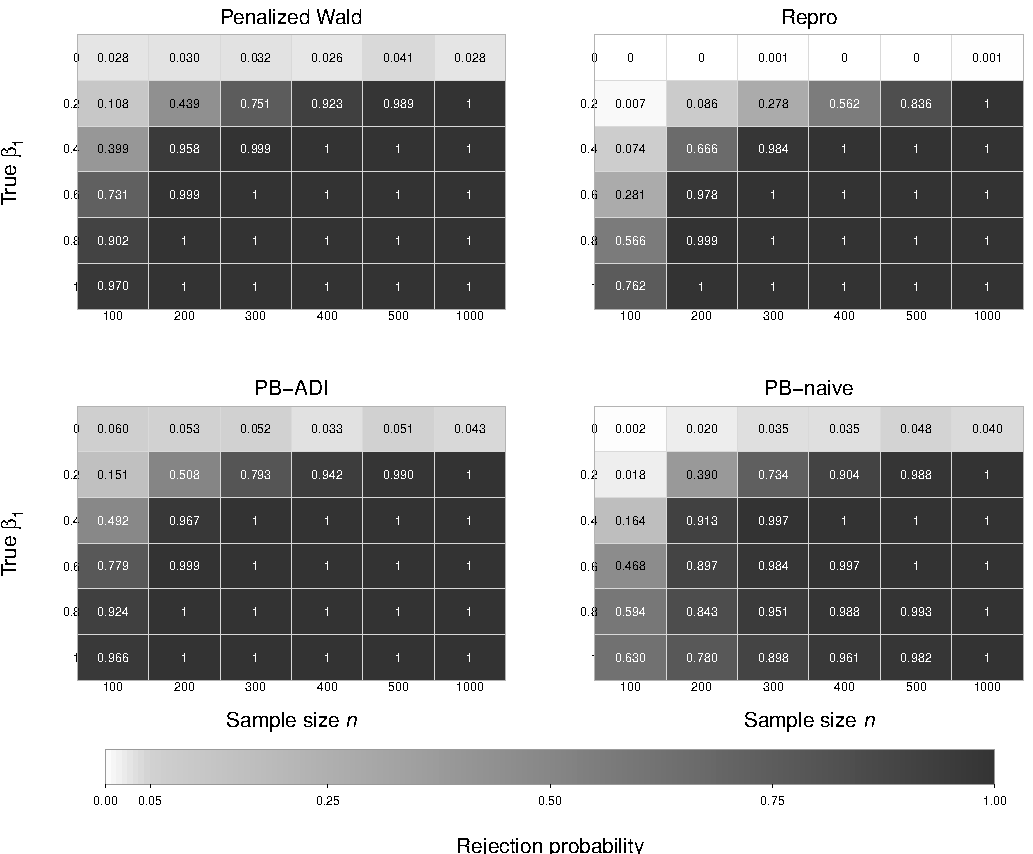
\includegraphics[width=0.95\linewidth]{results/figures/fig_exp2_grid.pdf}
\caption{Experiment 2. Rejection probability of $H_0:\beta_1=0$ at the $0.05$ level. Rows are the true slope, columns the sample size. The grey scale runs from $0$ to $1$ and breaks at $0.05$, so cells at or below the nominal level are light and cells above it dark: the bottom row of each panel is empirical size and the rest is power. \textsc{repro} is the procedure of \citet{awan2025simulation}; \textsc{pb-adi} and \textsc{pb-naive} are the debiased and naive parametric bootstraps as reported by \citet{wang2025optimal}.}
\label{fig:exp2-grid}
\end{figure}
